\section{DUNE Data Characteristics}
\subsection{Overview}

A number of parameters from DUNE/LBNF requirements, design documents,  and studies are used  as input
for estimations of the data rates in DUNE.
%In cases when derived parameters need to be generated based on these inputs this is accomplished using
%the software package \textit{dune-params}\cite{duneparams}
%developed specifically for this purpose. As the inputs and estimations are refined the results presented in this annex can be regenerated at will.
Buffering, triggering and readout strategy and algorithms of the DAQ
are complex R\&D items and are far from their final design and state of
readiness at the time of writing. Same applies to various analysis software.
For that reason, the data rate estimations involve some broad assumptions
and leave open some choices. This is described in more detail in the following subsections.

DUNE contains a number of major detector subsystems. The Liquid Argon TPC will present most challenges from
the standoint of real-time data processing and triggering, and can potentially dominate the data volume.
It incorporates the Photon Detector (PD) which while important produces less data so it won't be our focus
for the purpose of the data rate and volume estimates. There is also the Near
Detector Systems (see~\ref{sec:nds-params}).

\subsection{DUNE Detectors and Subsystems}

\subsubsection{Fundamental Parameters of the LArTPC}
\label{sec:fundamental-parameters}

The fundamental TPC parameters most relvant as input to the data rate estimations are summarized in
table~\ref{tab:fundamental-parameters}.

\begin{table}[ht!]
	\centering
	\begin{tabular}{| p{2.5in} | p{1in} |}
		\hline
		\textbf{Parameter} & \textbf{Value} \\ \hline
		Full height (single module) & 12.0\,m \\ \hline
		Full width (single module) & 14.5\,m \\ \hline
		Full length (single module) & 58.0\,m \\ \hline
		\# of detector modules & 4 \\ \hline
		\hline
		channels per APA & 2,560 \\ \hline
		APAs per module & 150 \\ \hline
		Active height (APA) & 6.0\,m \\ \hline
		Active width (APA) & 2.3\,m \\ \hline  \hline
		Drift distance in Liquid Argon & 3.6\.m \\
		\hline
		Drift velocity & 1.6\,mm/$\mu$s \\ \hline
		Drift time & 2.25\,ms \\ \hline
		\# drifts/readout factor & 2.4 \\ \hline
		readout time & 5.4\,ms \\ \hline \hline
		bytes/sample & 1.5 \\ \hline
		sample rate & 2.0\,MHz \\ \hline
		samples/readout & 10,800 \\
		\hline \hline
		Total \# of channels & 1,536,000 \\
		\hline
	\end{tabular}
	\caption{Fundamental parameters of DUNE Far Detector LArTPC.}
	\label{tab:fundamental-parameters}
\end{table}

Two of the parameters listed above (``drifts/readout'' and ``readout time'') need an additional comment.
The nominal readout time of 5.4ms is chosen such that additional time windows are covered just before and just
after the nominal $t_0$ (trigger) window. The value of 5.4\,ms is 2.4 times larger than the nominal drift of 2.25\,ms,
and it's listed in the table as the ``drifts/readout'' factor. This factor is not calculated precisely but was chosen based
on the experience with the 35t prototype (Sec.\ref{sec:35t}). The motivation behind this exta readout it to capture
potential activity in the TPC just before and just after the event of interest, so as to characterize this extraneous
ionization which for example can manifest itself as track segments due to cosmic rays background. It is quite
possible that the readout time will be revised as the final detector design is progressing, however the value of 5.4\,ms
was fixed in this document as nominal, in order to provide consistency of various estimates related to the data.

\subsubsection{The Photon Detector}
\label{sec:pd}
The Photon Detector (PD) which is built into the Far Detector LArTPC takes advantage of the fact that Liquid Argon
is an excellent scintillating medium.
The most significant requirements for the PD include determination of $t_0$ of an event relative to the TPC timing ---
resolution better than 1\,$\mu$s (event position resolution along drift direction of a few mm), and sufficient light
collection efficiency to allow triggering on neutrinos coming from a supernova, with the capability of detecting neutrinos with energies as
low as 20\,MeV.

Light produced by Liquid Argon Stintillation is collected from the TPC volume by the wavelength shifter and transported
by the light guide to the Silicon Photo-Multiplier (SiPMs) mounted at its end. A single whole assembly is mounted on each  APA frame.
The SiPMs are read out using shielded twisted-pair cables and the signal is passed to the module called SSP (the SiPM Signal
Processor). Digitized data is processed by a  Field-Programmable Gate Array (FPGA). The use
of the FPGA processing allows for a significant amount of customization of the SSP operation.


\subsubsection{The Near Detector Systems}
\label{sec:nds-params}
For sake of brevity, only basic information will be provided for the Near Detector Systems (NDS) which are under active development
at the time of writing and for which there is no final design yet. The main NDS components are:
\begin{itemize}
\item Near neutrino detector (NND), and its major component, the fine-Grained Tracker (FGT)
\item Beamline Measurement System (BLM)
\end{itemize}
\ 
In the reference design at the time of writing, a Fine-Grained Tracker (FGT) near detector consists of a straw-tube
tracking detector (STT) and electromagnetic calorimeter (ECAL) inside of a 0.4\,T dipole magnet.
In addition, Muon Identifiers (MuIDs) are located in the steel of the magnet, as well as upstream
and downstream of the STT. The FGT is designed to make precision measurements of the neutrino
fluxes, cross sections, signal and background rates at the percent level. Some basic parameters of the
NDS are presented in Table~\ref{tab:nds-params}.
\begin{table}[ht!]
\centering
\begin{tabular}{| p{1in} | p{1in} | p{1in} |}		\hline		
\textbf{Detector} & \textbf{Mass} & \textbf{Channels} \\ \hline
SST & 8t & 215,040 \\ \hline
ECAL & 93t & 52,224 \\ \hline
MuID & 100t & 165,888 \\ \hline
\end{tabular}
\caption{Main parameters of the Near Detector Systems}
\label{tab:nds-params}
\end{table}

The Beamline Measurement System (BLM) will be located in the region of the Absorber Complex
at the downstream end of the decay region to measure the muon fluxes from hadron decay.
It is not anticipated to produce large amounts of data when compared to other detectors in DUNE.

\subsection{Considerations for the Far Detector LArTPC Data}

\subsubsection{Sources of Data in the TPC}

Data being read out from the TPC are the result of a few different classes of interactions and other phenomena,
as outlined in table~\ref{tab:dune-data-sources}. Characteristics of these sources will
be a major factor influencing the rate and volume of data produced in DUNE.
\begin{table}[ht!]
	\centering
	\begin{tabular}{| p{1in} | p{4.5in} |}
		\hline
	\textbf{Type} & \textbf{Description} \\ \hline
		
	in-spill & Any activity in the detector which is coincident with
	the passage of beam neutrinos through the detector \\ \hline
	
	with-beam-$\nu$ & A subset of \textit{in-spill} where activity is
	consistent with a beam-$\nu$ interacting in the detector \\ \hline
	
	cosmic-$\mu$ & Activity due to the passing of cosmic-ray muons
	through the detector \\ \hline
	
	radioactivity & Activity due to the decay of radioactive
	isotopes \\ \hline
	
	atm-$\nu$ & Activity consistent with interactions from
	atmospheric neutrinos \\ \hline
	
	noise & Electronics noise (common-mode not considered) \\ \hline

	\end{tabular}
	\caption{Sources of data in the LArTPC.}
	\label{tab:dune-data-sources}
\end{table}

Not included in this table are two of the more exotic sources of signal, the Supernova Burst and Nucleon decay.
Due to their rare (and generally speaking, potential) occurance they will be considered separately as needed.


\subsubsection{Segments of the Dynamic Range of the TPC signals}

Signals produced by individual wires in the DUNE TPC will have a substantial
dynamic range. For example, $\beta$-decay of naturally occurring isotope $^{39}$Ar has the endpoint of
565\,keV, whereas signals due to interactions of energetic neutrinos can produce signals
equivalent to a few MeV energy deposition in a given channel depending on the event topology.

Each segment of the dynamic range will reflect certain types of events and this
be characterized by a respective data rate. For a systematic approach to estimates
and to reflect the physics of the detector,
it is helpful to consider three such segments when characterizing the LArTPC data and describe
them in terms of ``thresholds'' that may be applied to signals on ``per-wire'' basis and which can be
defined for example
in terms of ADC values (reflecting the collected charge, which can be translated to units like MeV with proper calibration).
%Optimizing these thresholds
%for optimal detector performance will require additional studies, so here they are used simply
%to distinguish separate domains of the signal dynamic range and to provide benchmarks for the data
%rate estimations. The data produced at each threshold are termed:
Using this concept the dynamic range can be considered with three distinct settings:
\begin{description}
	
\item[full-stream] The full-stream (FS) threshold means \textit{there is no threshold at all}, i.e.
FS data is effectively read out in every time bin (as defined by the ADC clock) and from every channel.

\item[zero-suppressed] The zero-suppression (ZS) threshold is an ADC value (in a single time bin,
on a single wire) roughly corresponding to ionization charge due to a 0.5\,MeV energy deposition.
All bins with ADC counts below this threshold are discarded from the data stream.

\item[high-energy] A high-energy (HE) threshold is assumed to be high enough so that
  that all electronics noise signals from radioactive decays are suppressed but low
  enough to not impact activity from beam neutrino interactions or potential nucleon decay activity.
  Further studies are needed to determine this threshold but currently
  it is taken, without rigor, to be 1$\div$10\,MeV.

\end{description}

The categories thus introduced will be considered in more details in the following sections, for example
see \ref{sec:zs-data} for a discussion of Zero Suppression and \ref{sec:ar39decays} for a discussion of
$^{39}$Ar decays rejection.


\subsubsection{Full-stream Data}

Full-stream (FS) data corresponds to reading all data in every ADC channel without
application of any threshold. Estimating the corresponding rate is a calculation based on
known parameters as it does not depend on the activity in the detector or the noise
level of the electronics. As its name implies, it is the most voluminous type of data
that can be generated by the TPC. The parameters which apply to this data are given in
table~\ref{tab:full-stream-parameters}.

\begin{table}[ht!]
	\centering
	\begin{tabular}{| p{3in} | p{1.1in} |}
		\hline

	\textbf{Parameter} & \textbf{Value} \\ \hline
	
	Bytes per sample & 1.5 \\ \hline
	
	DAQ sample rate & 2.0\,Mhz \\ \hline
	
	Channels per APA & 2,560 \\ \hline
	
	Number of APA per detector module & 150 \\ \hline
	
	Number of modules & 4 \\ \hline
	
	Total channels in DUNE & 1,536,000 \\ \hline \hline
	
	Drifts per readout & 2.4 \\ \hline
	
	Drift time & 2.25\,ms \\ \hline

	Total readout window & 5.4\,ms \\ \hline \hline
	
	Beam spill repetition rate & 0.83\,Hz \\ \hline
	
	Annual run time fraction & 0.667 \\ \hline
	\end{tabular}
	\caption{Parameters pertaining to full-stream data rates.}
	\label{tab:full-stream-parameters}
\end{table}
The expected data rates for FS data are given
in table~\ref{tab:full-stream-volume}.
\begin{table}[ht!]
	\centering
	\begin{tabular}{| p{3in} | p{1.1in} |}
		\hline	
	
	\textbf{Parameter} & \textbf{Value} \\ \hline
	Full-stream readout size & 24.9\,GB \\ \hline
	Full-stream 1 year in-spill data volume & 436\,PB \\ \hline
	Full-stream 1 second data volume & 4.6\,TB \\
	Full-stream 1 minute data volume & 276.5\,TB \\	\hline
	Full-stream 1 year data volume & 145.4\,EB \\ \hline
	\end{tabular}
	\caption{Data volumes and rates for full-stream data acquisition.}
	\label{tab:full-stream-volume}
\end{table}
The first row gives the data size corresponding to one DAQ readout cycle (5.4\,ms, as explained in \ref{sec:fundamental-parameters}).
The second is appropriate for any strategy that intends to record FS data for each beam spill.
The third contains two numbers that characterize data volume relevant to a strategy which aims
to record FS data for Supernova Burst candidates. The final row  shows the total annual data
volume that the DUNE DAQ is capable of producing (purely in theory).
\textit{These numbers are not meant to imply ongoing recording of full-stream
data to permanent storage} and are only given to better define the problem and initial parameters
of recording data in DUNE.


\subsubsection{Potential capabilities of the Far Detector TPC DAQ system}
For more detail on the DUNE Data Acquisition see Section~\ref{sec:daq}. One of its central components
is an array of \textit{Reconfigurable Cluster Elements} (RCE)~\cite{slac_rce_1}, which offer very high
readout speeds, considerable real-time computing power and enable flexibility of system configuration.

In addition to considerations of various signal sources, the data rate estimates depend on capabilities of the DAQ system,
in particular as they apply to data compression and rejection of radiological background.
Examples of relevant DAQ capabilities to be considered are:

\begin{itemize}

\item Identification by the DAQ trigger farm of small and scattered regions of isolated activity
  consistent with $^{39}$Ar decays in order to suppress these data.

\item Ability of the RCEs to apply zero suppression algorithms
with a given threshold to real-time data sent to the trigger farm.

\item Trigger-specific zero suppression algorithms and thresholds to be applied
in the RCEs to the data sent to the data farm.

\item Possibility of RCE-local data storage (e.g. to serve as a buffer for near-time SNB trigger decision).

\item Detection of Regions of Interest (ROI) for high-threshold events, e.g. identifying the APAs
which register the signal of an energetic lepton resulting from a beam neutrino interaction, so as
to avoid collecting and writing the data from ``empty'' parts of each TPC module.

\end{itemize}

Based on the current understanding of progress in DAQ R\&D, it is reasonable to assume at the time of
writing that the above DAQ characteristics will indeed be implemented in DUNE.




\subsubsection{Zero-suppressed Data}
\label{sec:zs-data}
The Far Detector LArTPC is expected to operate is very low background conditions. In practice
is means that in each instance the signals of interest (such as induced by reactions of beam neutrinos)
will only present in a fraction of channels.
There are options in choosing the exact zero-suppression (ZS) procedure,
and the final choice has not been made. The simplest procedure may be implemented
as follows: in each channel, all digitized time bins in which the ADC
values are below the given threshold are removed. More discussion on possible alternative
ZS methods and their impact on the data rate are given below.

The nominal ZS threshold is assumed to be the ADC counts equivalent to 0.5\,MeV energy deposited as
ionization which is collected by a single wire.
It is assumed that the application of zero-suppression at this
threshold completely removes ADC counts due to just noise.
% although an estimate of data rates due to noise is given.
Estimations of different sources of ZS data are summarized in table~\ref{tab:zs-volume}.

In order to better preserve the shape of the signal waveform digitized and recorded for
each channel, a more complex strategy may be applied where the data is accepted in additional
time windows before and after the ``main'' pulse which exceeds the nominal ZS threshold. This
is a subject of R\&D at the time of writing. Obviously, implementation of such scheme will lead
to an increase in the recorded data volume compared to minimalistic version. Assuming that
each extra window is comparable in duration to the peak of the signal above the threshold,
a rough estimate is that this factor could be up to a factor of 2 and mey be 3. However, given
that the design of this and other compression algorithms is still ongoing, and for better consistency
and ease of reference, this is not included in the ZS data estimates presented Table~\ref{tab:zs-volume}
and in the following sections. Also not included is lossless data compression that may be applied
in addition to the lossy ZS algorithm (see \ref{sec:data-compression}).

	
\begin{table}[ht!]
\centering
\begin{tabular}{| p{1.2in} | p{0.9in} | p{0.75in} | p{1in} | p{0.9in} |}		\hline		
Source & Event Rate & Event Size & Data Rate & Volume/year \\ \hline
all $^{39}$Ar & 11.2\,MHz & 150\,B & 1.6 GB/s &  53\,PB \\ \hline
all in-spill & & & & 159\,TB \\ \hline
with-beam-$\nu$ & & & & 79\,GB \\ \hline
cosmic-$\mu$ & 0.259\,Hz &2.5\,MB & 647.4\,kB/s & 20\,TB \\	\hline
beam-$\nu$ & 8770\,year$^{-1}$ & 2.5\,MB & 0.69 kB/s & 22 GB \\ \hline
SNB cand. (ZS) & 12 year$^{-1}$ & 16.7\,GB & 6366\,B/s & 201\,GB \\ \hline
SNB cand. (FS) & 12 year$^{-1}$ & 46.1\,TB & 17.5\,MB/s & 553\,TB \\ \hline
\end{tabular}
\caption{Data rate estimations for ZS data from various sources.
An additional FS data estimation is given for supernova burst (SNB).}
\label{tab:zs-volume}
\end{table}

\subsubsection{$^{39}$Ar Decays}
\label{sec:ar39decays}
Decays of naturally occurring isotope $^{39}$Ar could potentially dominate the data volume.
The end point of the $^{39}$Ar decay is at 565\,keV and about
25\% of the beta spectrum is above the ZS threshold \cite{ar39endpoint}.
The expected total decay rate is 1.0 hertz per kilogram \cite{ar39bkg}.

Ionization due to $^{39}$Ar decays is very localized and it is reasonable to assume
that spatial dispersion of the charge will be no larger than the wire pitch,
and for the most part no larger than the distance drifted during the time span
corresponding to one ADC sample.
Based on the likely value of shaping time to be set for the electronics (1-3\,${\mu}s$),
the resulting waveform will be spread over $\sim$10\,$\mu$s or $\sim$20 samples. Because offline signal
processing is sensitive to tails of waveforms, even more time samples may be required.
Finally, it is assumed that due to localization of charge a single collection wire and two induction
wires in each view will register an appreciable signal.

Based on preliminary estimates such as given in table~\ref{tab:zs-volume},
due to scale of the DUNE TPC the $^{39}$Ar decays generate a very large volume of data, recording which
is not justified given their relative lack of physics importance.
Some mitigation is required and will be developed. The simplest solution is to increase the ZS
threshold to be above the decay endpoint.
This may have a negative effect on detector performance due to removing small energy
depositions associated with larger events and thus will only be
considered if absolutely required to mitigate the rate.

A better approach is the one that drives the requirement on the DAQ
that the trigger farm be capable of identifying isolated activity
consistent with $^{39}$Ar on a per-APA basis in order to veto its
recording. The DAQ is expected to be able to provide this functionality.
This then leaves $^{39}$Ar which is accidentally coincident in the
same APA with readouts from other activity such as beam-$\nu$
interaction and cosmic muons.
The annual number of above ZS-threshold $^{39}$Ar decay events
coincident anywhere in the DUNE detector with beam-$\nu$ activity is
given in table~\ref{tab:zs-volume} as 79\,GB. Of that only 3\% are coincident
in the same APA bringing the added data rate to about 10\% that of the beam-$\nu$ activity.

\subsubsection{Supernova Burst}

The Supernova Burst (SNB) data is estimated assuming a
\textit{false-positive} SNB rate of 12 year$^{-1}$ and a readout time of
10s. It should be emphasized that both these parameters are subject to
modification and are used simply to provide benchmark examples.

The SNB events are predicted to have a unique signature whereby
neutrino interactions will produce on order of 1000 events across
the Far Detector modules over a time around ten seconds and with a
neutrino spectrum up to 100MeV. Under this circumstances, 
the most likely source of a false positive SNB trigger may be an upward
fluctuation in the registered rate of $^{39}$Ar decays.
It can therefore be assumed that the data volume of a
false-positive SNB trigger is dominated by $^{39}$Ar decays.

In order to ensure optimal efficiency of detection for the SNB neutrinos,
an  additional trigger stream must be put in place in which
reduction of $^{39}$Ar background (such as described in \ref{sec:ar39decays}) will not be employed, as it would potentially impact the SNB neutrinos. Hence, this background 
will dominate the data volume. The data volume due to the SNB events themselves is not significant.

Further, a lower ZS threshold may be considered for saving such
candidate SNB occurrences. The possible data rate of SNB candidates is thus bound by the nominal
ZS $^{39}$Ar rate and the FS rate. The exact strategy for saving SNB candidates requires additional study
and may have implications on DAQ hardware.

\subsubsection{Noise}

% fixme: is this remotely true?
The nominal ZS threshold of 0.5MeV is based on an older requirement of a
9:1 signal to noise ratio for a 1 MIP. The most likely MIP is 1.8MeV$\times$cm$^{-1}$ or 0.9 MeV per wire pitch.
This implies an RMS noise requirement equivalent to 0.1 MeV and then the 0.5 MeV equivalent ZS
threshold represents a $5\sigma$ cut. Across the 1,536,000 channels and the 10,800 samples
per readout this gives about 5,000 samples above the nominal ZS threshold. Their distributed
nature and isolated pattern of appearance make them subject to the same rejection criteria as
$^{39}$Ar, therefore this factor can be ignored for the purposes of data volume estimates.


\subsubsection{High-energy Threshold}

For the purpose of these estimates the  high-energy (HE) threshold is chosen at the level above 
the energy scale of the radiological backgrounds relevant for the LArTPC, and set at  10.0MeV.
A more careful study is needed to determine a potentially more optimal value for this threshold.
The data rates with the HE threshold applied are summarized in table~\ref{tab:he-volume}.

	
\begin{table}[ht!]
\centering
\begin{tabular}{| p{1.2in} | p{0.95in} | p{0.75in} | p{1in} | p{0.9in} |}		\hline	
Source & Event Rate & Event Size & Data Rate & Volume/year \\ \hline
$^{39}Ar$ & - & - & - & -\\	\hline
cosmic-$\mu$ & 0.259Hz & 2.5MB & 647.4 kB/s & 20TB \\ \hline
beam-$\nu$ & 8770 year$^{-1}$ & 2.5MB & 0.69 kB/s & 22GB \\
\hline
SNB cand. & - & - & - & -\\ \hline
\end{tabular}
\caption{Data rate estimations for data from activity above the high-energy (HE) threshold from
various sources.}
\label{tab:he-volume}
\end{table}


%\input{annex-rate/generated/he-volume-table}

With the HE threshold in place, activity from the $^{39}$Ar events and any SNB
candidates will not be visible (i.e. will be rejected in DAQ). Although actual SNB
events may result in neutrino with energies as high as 100MeV applying such a high
threshold to SNB candidates won't be optimal and is not being considered at this point.
For this reason, contribution from SNB to these data is not calculated for this threshold setting.


\subsubsection{Compression}
\label{sec:data-compression}

The above estimates assume that the only method of data volume reduction to be employed is the
lossy compression by removal of data below some threshold.

\begin{figure}
%[h!]
	\centering
	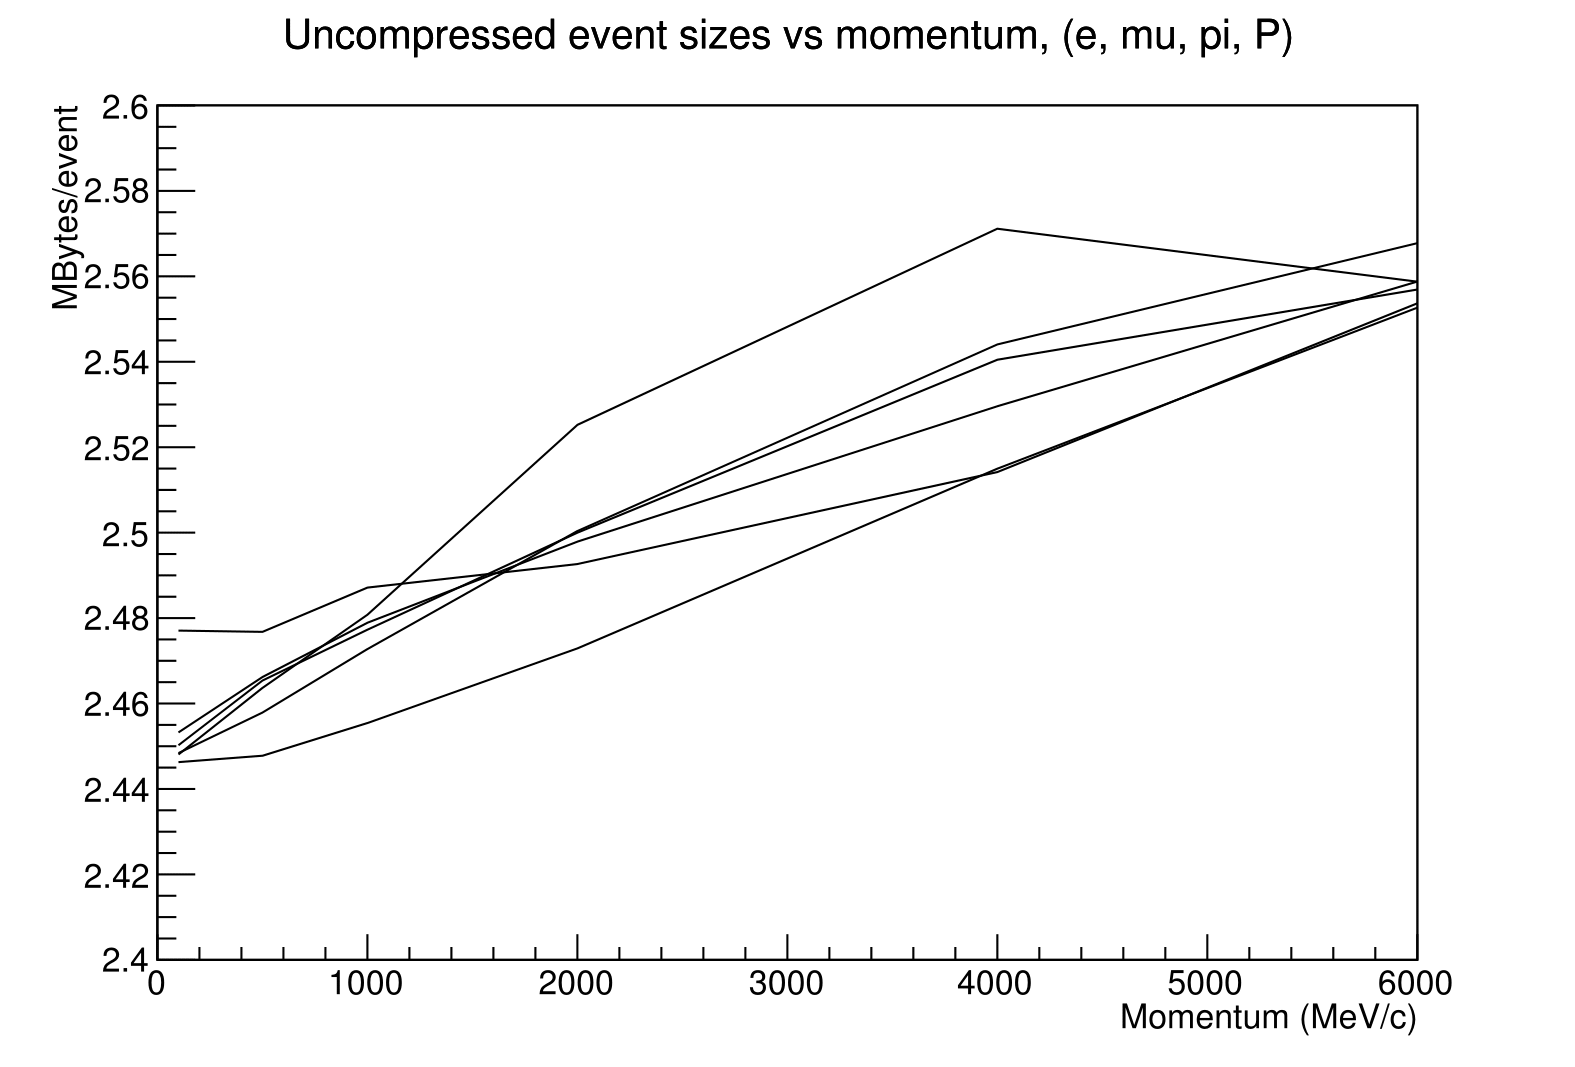
\includegraphics[width=0.6\textwidth]{btot.png}
	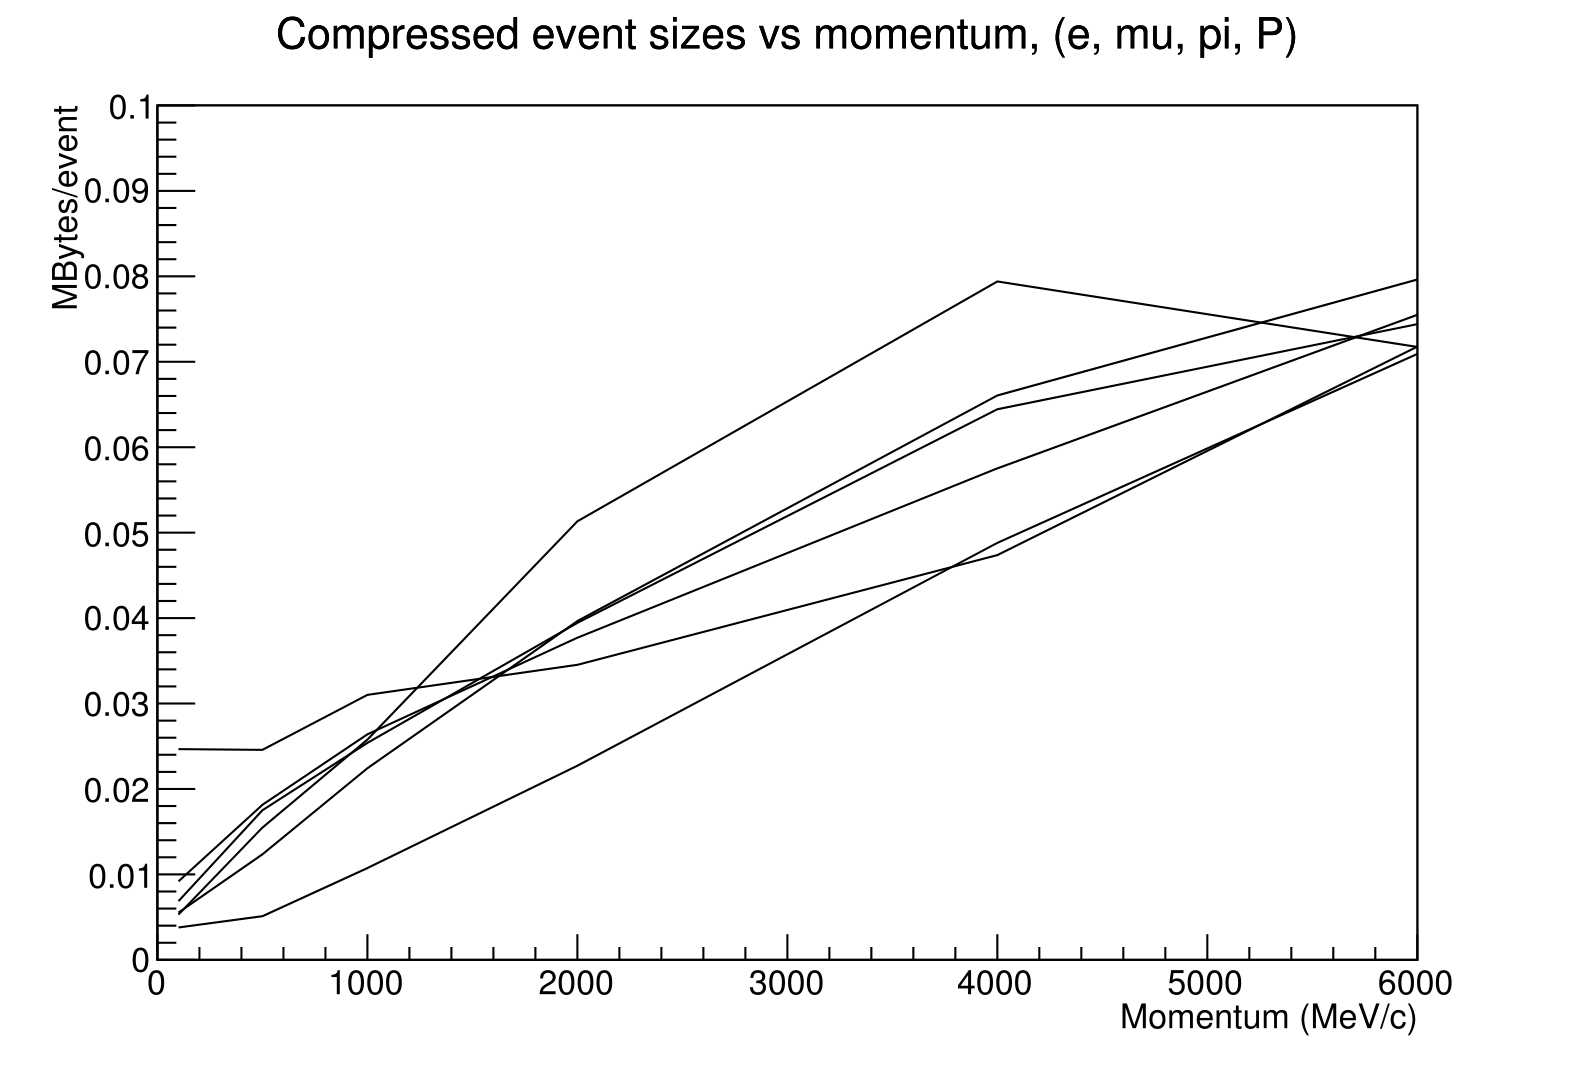
\includegraphics[width=0.6\textwidth]{bzip.png}
	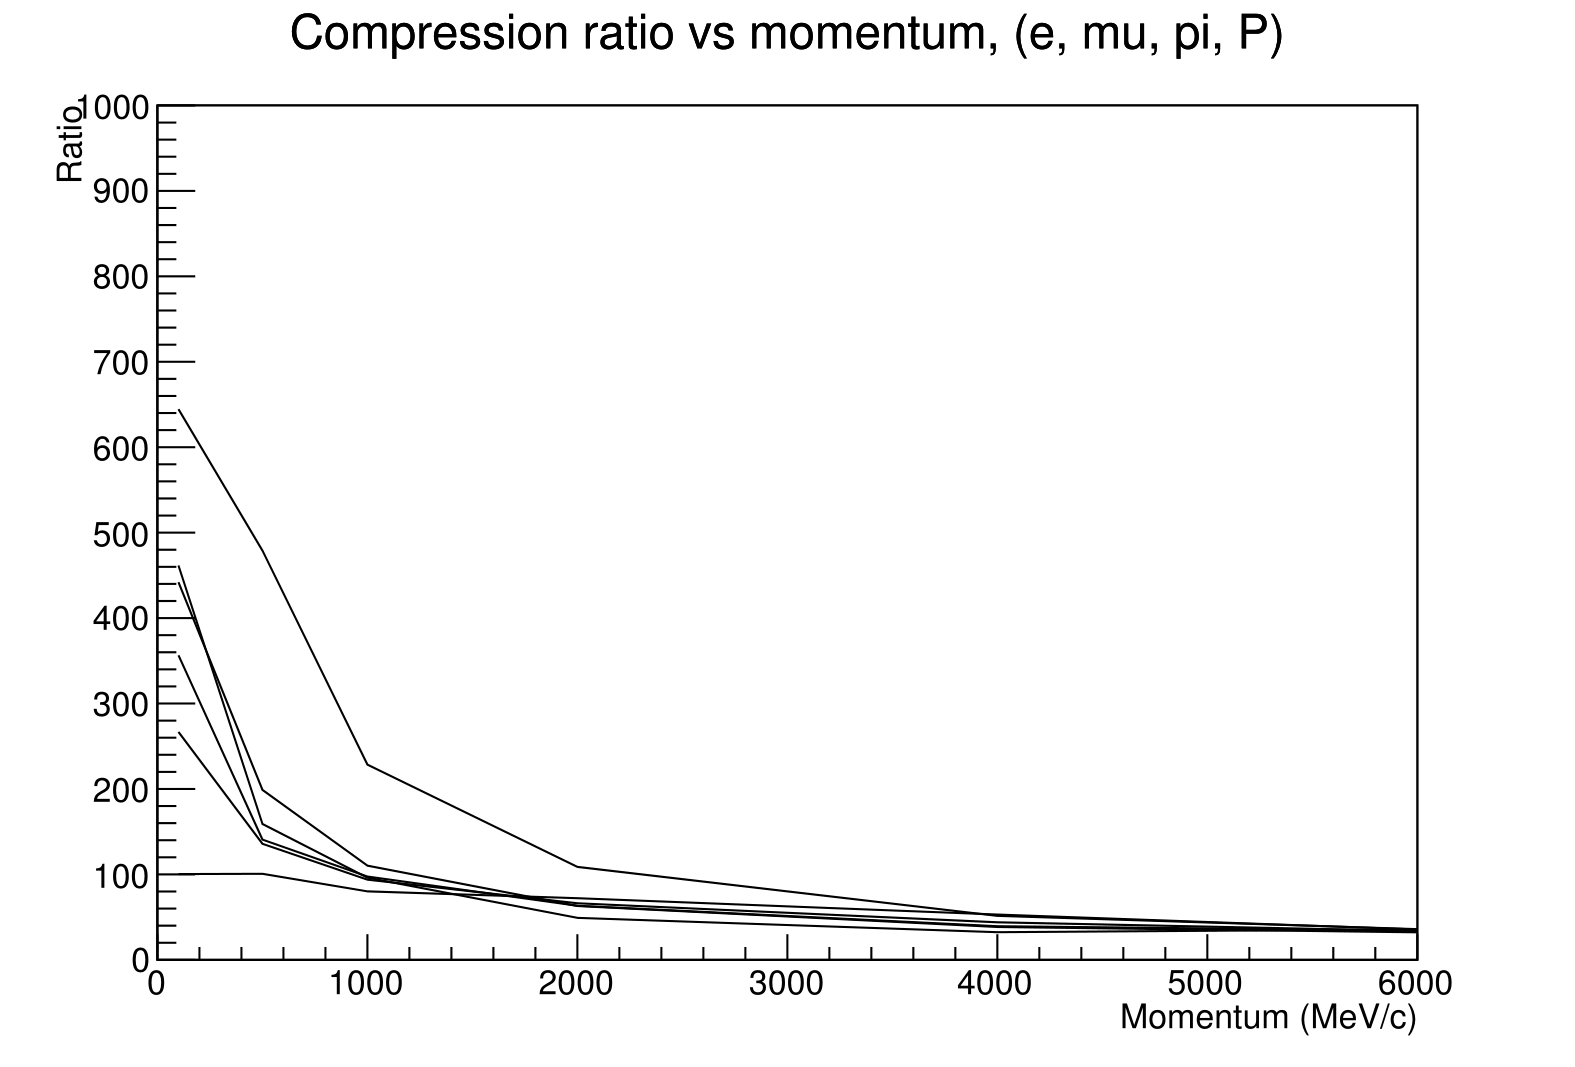
\includegraphics[width=0.6\textwidth]{brat.png}
	\caption{Estimation of DUNE zero-suppressed event sizes for different particles and momenta before (left) and after (center)  compression and their ratios (right).}
	\label{fig:data-compression}
\end{figure}

However, in addition to that
a lossless compression is possible. For example, the DAQ system can employ Huffman encoding
during readout, or compression features built into ROOT may be used during writing data to files. In order to estimate
the effects of compression, specific particle types and energies were simulated using LArSoft.
The initial kinematics for the simulated samples covered a matrix of
particles ($e$, $\mu$, $\tau$, $\pi^+$, $\pi^-$, $\pi^0$ and proton) and momenta
(100MeV to 6GeV).
The uncompressed and compressed sizes are summarized in figure~\ref{fig:data-compression}.


%\begin{cdrfigure}[Event size estimations.]{data-compression}{Estimation of DUNE zero-suppressed event sizes for
%    different particles and momenta before (left) and after (center)
%   compression and their ratios (right).
%   Each line represents one particle type.
%    The samples were generated with LArSoft assuming
%   10 kilo tonne detector module with 300000 channels.}

%  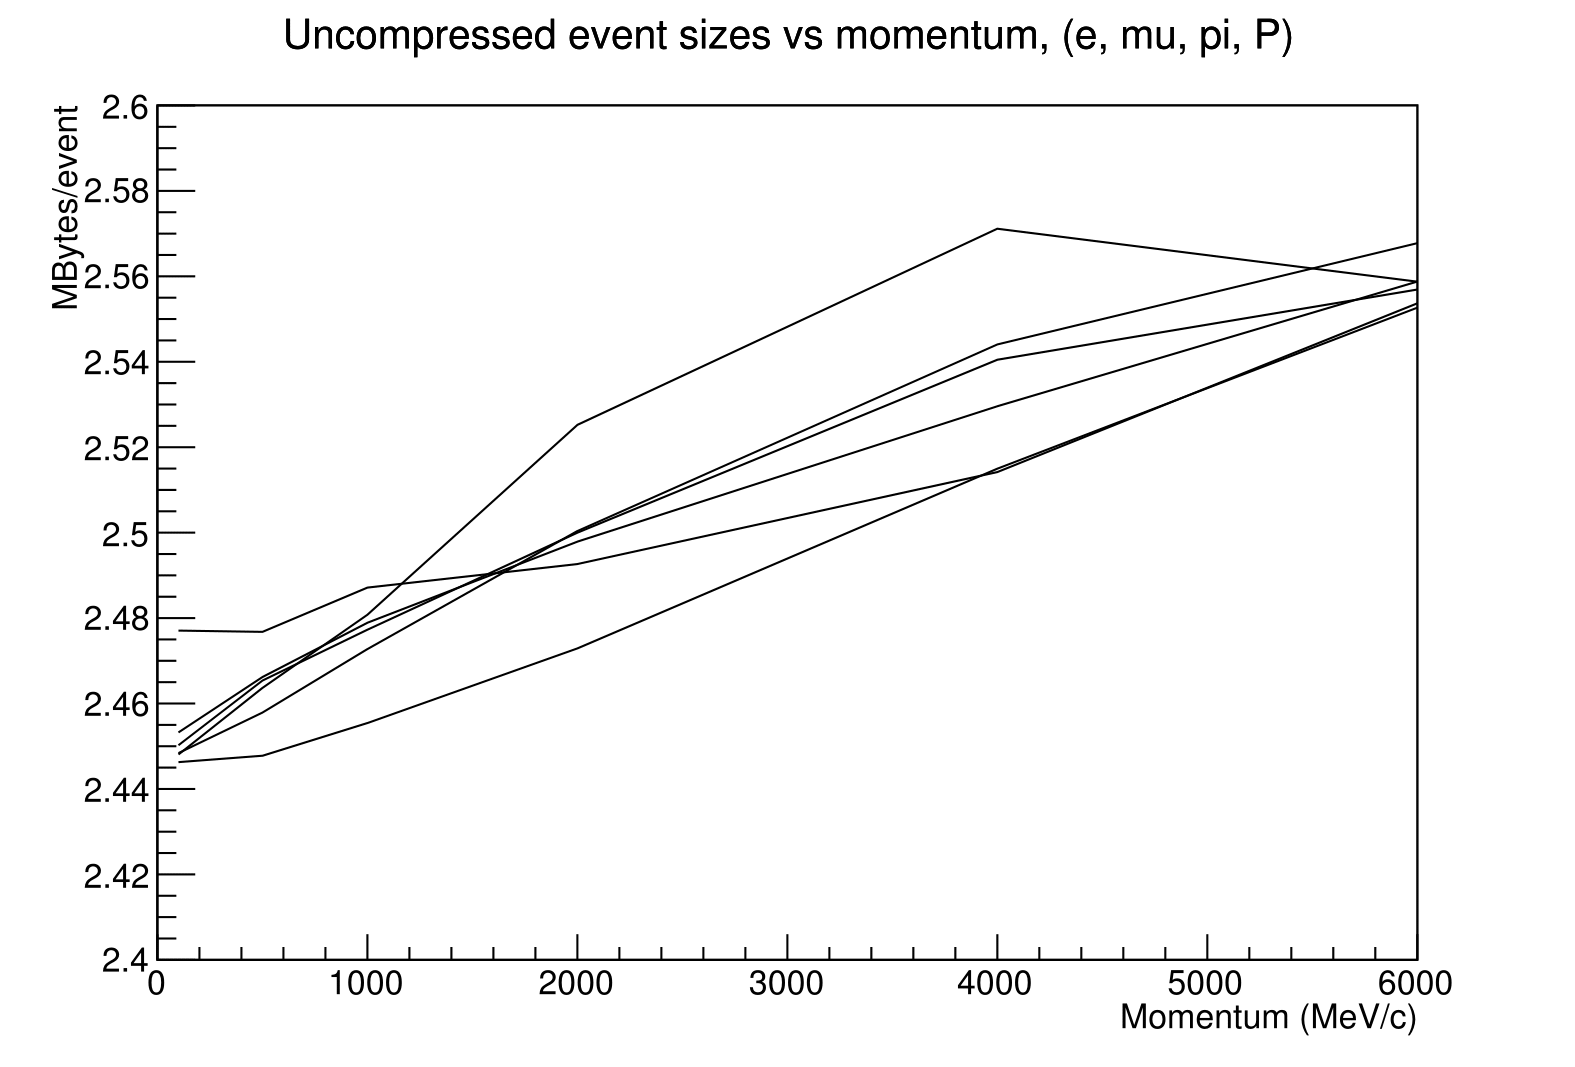
\includegraphics[width=0.3\textwidth]{btot.pdf}
%  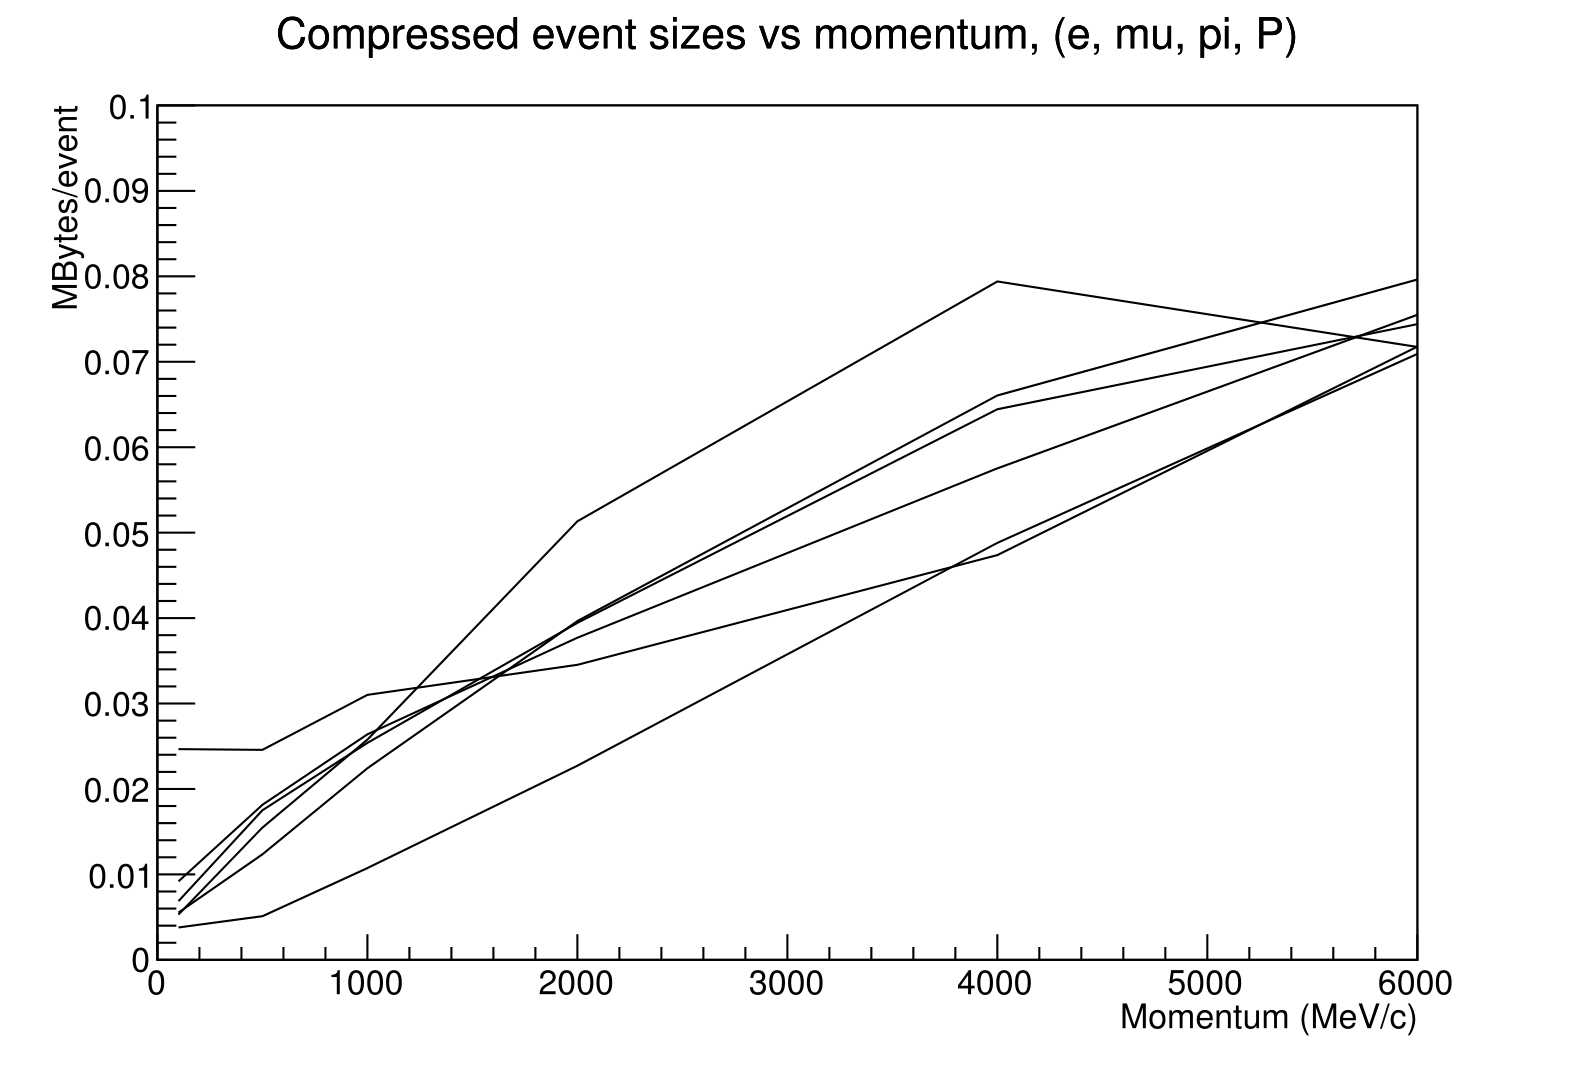
\includegraphics[width=0.3\textwidth]{bzip.pdf}
%  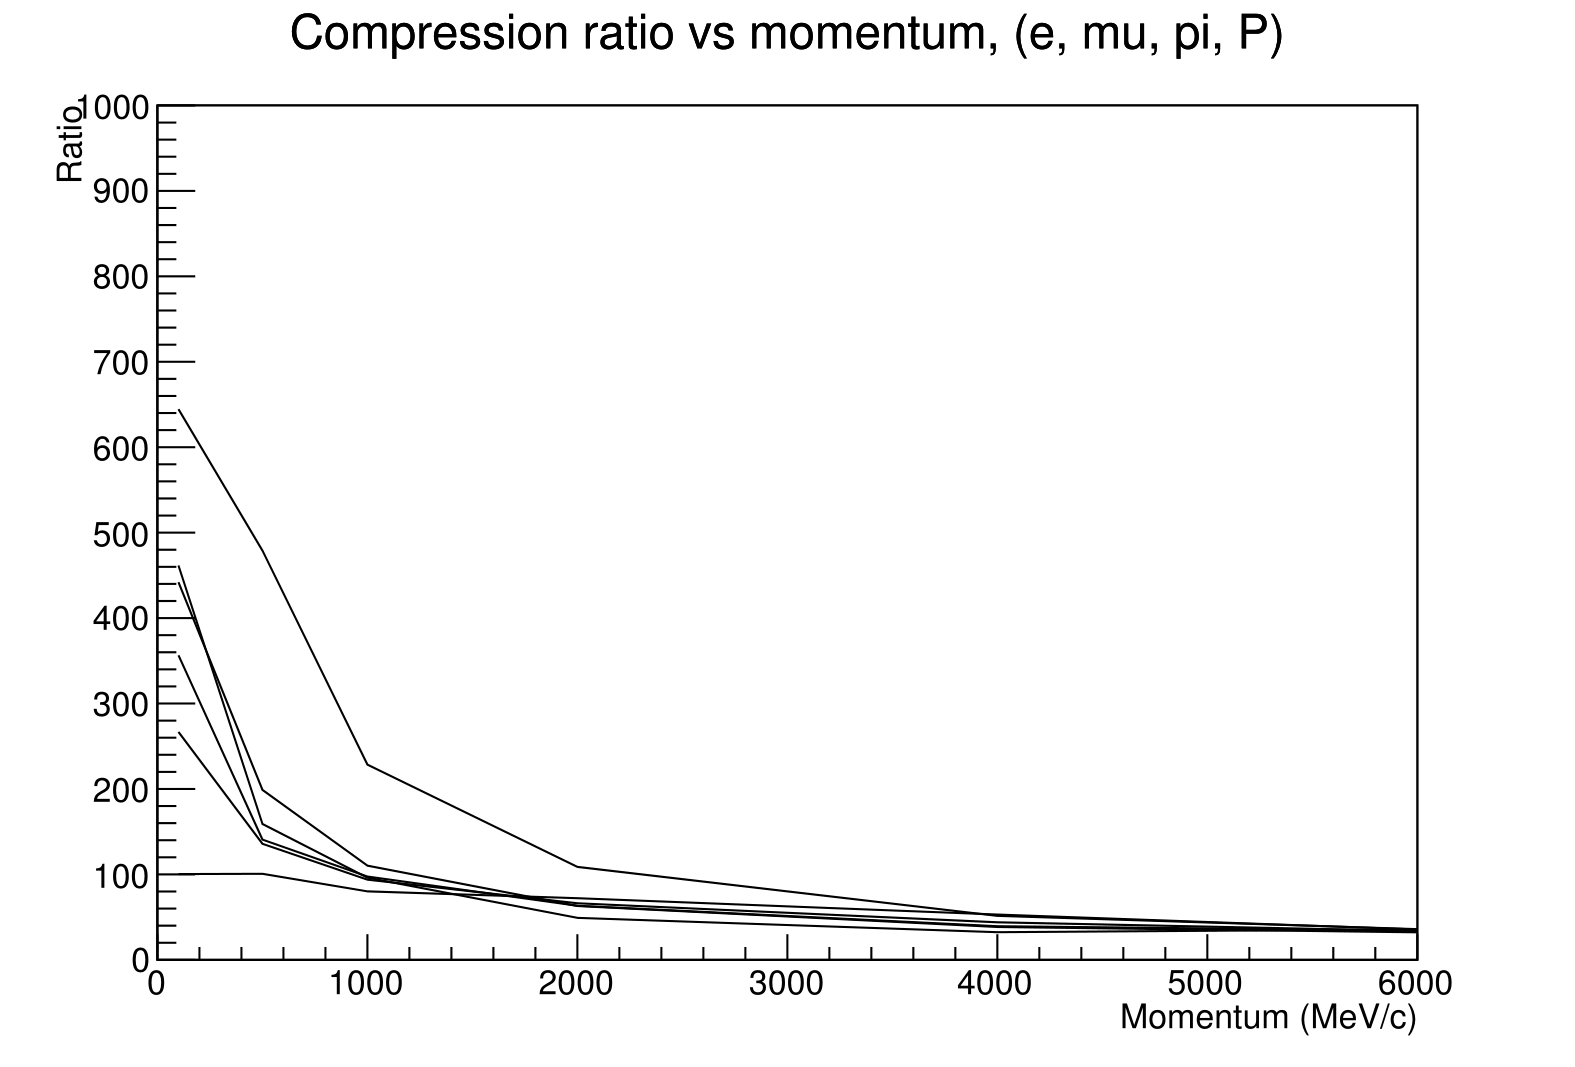
\includegraphics[width=0.3\textwidth]{brat.pdf}

%\end{cdrfigure}

It must be noted that this exercise discovered the bulk of the
compressed data written by LArSoft is actually made up channel ID
numbers providing a data inflation of about a factor of 10.
For uncompressed data this added about 50\%.
There are also additional data elements related in the ``raw data''
branch which are superfluous or at best repeated more frequently than
is likely to be required.
In the LArSoft output, even though zero suppression is applied, every
channel has an associated a pedestal and a sigma as well as a
compression number.
There is also a sample count in addition to the one in the sample
vector which is stored.
These values do no vary yet each take up about the same (uncompressed)
size as the ADC values and are significant in size even after
compression.
They are not included in figure~\ref{fig:data-compression}.

Finally, as can be seen in the figure, the change in uncompressed
event size is only a minor function of event momenta and particle types.
It is believed that LArSoft is saving additional overhead for all
channels, even those that have been fully zero-suppressed.

The simulation used a detector module consisting of 300,000 wires and thus naively the event
size in the full reference detector would be some 5 times larger.
However, given the arguments above, it is expected that this leads to
a gross over-estimate, possibly by one or two orders of magnitude from
what should be expected if even just a little effort is put into
designing a better storage schema.
Once compression is assumed, the problems with this sub-optimal
storage schema are lessened.
We then select the uncompressed event size to be beameventsize and
the compressed event size of 0.1\,MB based
on data presented in Fig.~\ref{fig:data-compression}.
We identify this with being the zero-suppressed data produced by just
activity due to beam interactions or similar energy events and accept
the large over-estimation as a generous safety factor.

\subsection{Considerations for the Near Detector Data}
At the time of writing, there are many parameters of the NDS that are yet to be well defined.
Table~\ref{tab:nds-event-rates} summarizes current estimates of the event rates
in the ND systems from various sources.

\begin{table}[ht!]
\centering
\begin{tabular}{| p{0.8in} | p{0.8in} |}		\hline		
\textbf{Source} & \textbf{Rate} (Hz)\\ \hline
Beam-$\nu$ & 40.2 \\ \hline
Rock & 10.0 \\ \hline
Cosmic & 0.04 \\ \hline
Total & 50.2 \\ \hline
\end{tabular}
\caption{Summary of combined DUNE Near Detector system event rate estimations.}
\label{tab:nds-event-rates}
\end{table}

Based on these rates and occupancy estimated in preliminary Monte Carlo Studies, the projected
data rate from the NDS will be in the megabytes per second range, and effectively well below
the levels characteristic of the Far Detector.
